\chapter{Physical Basis of Spectroscopy}
\label{ch:theory}

Astronomical spectroscopy can be seen as the study of emission and absorption lines against a background continuum. The material provided here omits much of the necessary physics background, but provides at least a basic introduction to spectroscopy.

\section{Spectral Lines}

\subsection{Transition Probabilities}

The Einstein coefficients are defined as the probabilities for spontaneous transitions (A for emission, and B for absorption). The inverse of these coefficients give the radiative lifetimes (e.g. 1/A is the time for a transition to spontaneously decay).
\begin{equation}
	A_{ji} = \frac{8 \pi h B_{ij} g_i}{g_j \lambda^3} \\
\end{equation}
\begin{equation}
	B_{ij} = \frac{f_{ij} e^2 \lambda}{4 \epsilon h c m_e}
\end{equation}
where $f$ is the oscillator strength, and $g$ the statistical weight of states $i$ and $j$ respectively. These equations treat the transition as if it were a bound harmonic oscillator, and asks how efficient the transition is at absorbing energy. Often, the $g$ and $f$ values are tabulated together:
\begin{equation}
	g_i f_{ij} = A_{ji} g_j \lambda^2 \left(\frac{4 \epsilon c m_e}{8 \pi e^2}\right)
\end{equation}
The oscillator strength is a transition probability which can be experimentally or theoretically derived from Quantum Mechanics. Typical A values are $10^8$--$10^9$~s$^{-1}$ for permitted resonance transitions, $\sim 10^3$~s$^{-1}$ for semi-forbidden lines, and $\sim 10^{-3}$~s$^{-1}$ for forbidden lines. Thus, forbidden lines are usually seen only in diffuse environments where the time between collisions is longer than about 1000 seconds.

\subsection{Local Thermodynamic Equilibrium}

The distribution of atomic states and energies for LTE is given by statistical mechanics. The Boltzmann equilibrium provides the relative number of atoms in an excited state, $j$, compared with the ground state ($j=1$) at a given temperature, $T$:
\begin{equation}
	\frac{N_j}{N_1} = \frac{g_j}{g_1} \exp\left(\frac{-\Delta E}{kT}\right)
\end{equation}
where $\Delta E$ is the energy difference between the ground and excited states, and $k$ is the Boltzmann constant ($k = 1.38 \times 10^{-16}$~erg~K$^{-1}$). The energies for hydrogen may be approximated by the empirical formula
\begin{equation}
	E_n = \frac{-h c R_H}{n^2} = -13.6{\textrm eV}\frac{1}{n^2}
\end{equation}

The energies of atoms will follow a Maxwell-Boltzmann distribution, which can be expressed as a function of either temperature or velocities:
\begin{equation}
	n(E) = \frac{2 N}{\pi^{1/2} (kT)^{3/2}} E^{1/2} \exp\left(\frac{-E}{kT} dE\right)
\end{equation}
which has a most probably energy $kT$, or a most probable velocity $v = \sqrt{(2kT/m)}$. However, LTE is not usually applicable to the interstellar medium (ISM), as low densities mean that a Boltzmann equilibrium is rarely achieved because collisions are too rare. In the ISM, therefore, radiative processes become important. The Maxwellian distribution is usually applicable to the ISM.

\section{Measuring Absorption and Emission Lines}

Lines are often measured via their equivalent width, $W$, using the relationship:
\begin{equation}
	W = \int{\frac{I_0 - I_{\lambda} d\lambda}{I_0}}
\end{equation}
where $I_0$ is the continuum intensity and $I_{lambda}$ the intensity at the wavelength $\lambda$. Note that, using this definition, emission lines will have negative $W$ whilst absorption lines will have positive $W$. Equivalent width can most easily be thought of as the area which would be taken up by the line on a normalized spectrum ($I_0 = 1$). In the case of observed spectra there will be noise, which will in turn lead to a detection limit. The n$\sigma$ detection limit is
\begin{equation}
	W_{\rm lim} = \frac{n \times d \times \sqrt{M}}{\rm SNR}
\end{equation}
where $d$ is the dispersion (pixel width in \AA), and $M$ the number of pixels across the line. In the case of unresolved lines, this can be approximated to
\begin{equation}
	W_{\rm lim} = \frac{n \times {\rm FWHM}}{\rm SNR}
\end{equation}

The width of a line is usually expressed in km/s as either the velocity dispersion ($\sigma$) or the FWHM. In the case of a Gaussian distribution the two quantities are related, with ${\rm FWHM} = 2\sqrt{2\ln2}\sigma = 2.355\sigma$. Widths are often expressed in terms of the Doppler width, $b$, caused by thermal and turbulent broadening, where:
\begin{equation}
	b = \sqrt{2}\sigma = \frac{\rm FWHM}{2\sqrt{\ln2}}
\end{equation}
For emission lines, the flux is often quoted instead of the equivalent width, either in units of $F_{\nu}$ (ergs s$^{-1}$ cm$^{-2}$ Hz$^{-1}$ (Jy)), or $F_{\lambda}$ (ergs s$^{-1}$ cm$^{-2}$ \AA$^{-1}$) where $F_{\lambda} = F_{\nu} c/\lambda^2$. Graphs may be plotted with $\lambda F_{\lambda}$, or total energy.

\section{The Voigt Profile}

Spectral lines are broadened by various processes, including pressure broadening (more important in stars), thermal and turbulent broadening, and natural broadening (which occurs due to Heisenberg's uncertainty principle $\Delta E \Delta t \geq \hbar$). Because any transition has a finite lifetime $\Delta t = 1/A_{ji}$, the natural width in terms of frequency is $\Delta \nu_{N} = A_{ji}/2\pi$. Often this natural frequency width is replaced by the damping constant $\Gamma = 2 \pi \Delta \nu_{N}$, which is connected to the radiative transfer probability: for a transition from the ground state, $\Gamma$ is the sum over the Einstein coefficients for spontaneous emission for levels up to the level in question. The absorption cross-section (measure of probability) for natural broadening can then be expressed as:
\begin{equation}
	\sigma_L(\nu) = \left(\frac{\pi e^2}{m_e c}\right)f\frac{\Gamma/4 \pi^2}{(\nu - \nu_0)^2 + (\Gamma/4\pi)^2}
\end{equation}
(ignoring the term for stimulated emission).

Thermal and turbulent motions are combined into the Doppler width, which is assumed to follow a Gaussian distribution.
\begin{equation}
	P(v) = \frac{1}{b \sqrt{\pi}}e^{-(v/b)^2}
\end{equation}
\begin{equation}
	b = \sqrt{b^2_{\rm thermal} + b^2_{\rm turbulent}} = \sqrt{\frac{2kT}{m} + b^2_{\rm turbulent}}
\end{equation}
If $b$ is dominated by thermal broadening, then this simplifies to $b = 12.8 {\rm km/s} \sqrt{T/m}$

Combining Equations 11 and 12 gives an absorption cross-section
\begin{equation}
	\sigma(\nu) = \left(\frac{\pi e^2}{m_e c}\right)f\frac{\Gamma}{4\pi^2}\int^{+\infty}_{-\infty}\frac{e^{-(v/b)^2}dv}{(\nu - \nu_0(1+v/c))^2 + (\Gamma/4\pi)^2}
\end{equation}
This expression can (fortunately) be simplified using the Voigt function, $H(a,u)$
\begin{equation}
	H(a,u) = \frac{a}{\pi}\int^{+\infty}_{-\infty}\frac{e^{-y^2}dy}{(u-y)^2 + a^2}
\end{equation}
where
\begin{equation}
	\Delta \nu = \frac{b\nu_0}{c}; a = \frac{\Gamma}{4\pi \Delta\nu}; u = \frac{c(\nu-\nu_0)}{\nu_0 b}; y=\frac{v}{b}
\end{equation}
Substituting this into Equation 14 gives
\begin{equation}
	\sigma(\nu) = \frac{\sqrt{\pi} e^2 f}{m_e c}\frac{H(a,u)}{\Delta \nu}
\end{equation}
We can now write the line optical depth ($\tau = N \sigma = \ln(I_0/I)$) as
\begin{equation}
	\tau(\nu) = \frac{\sqrt{\pi}e^2}{m_e}\frac{N f}{b\nu}H(a,u)
\end{equation}
or, written as a function of wavelength,
\begin{equation}
	\tau(\lambda) = \frac{\sqrt{\pi}e^2}{m_e c}\frac{N f \lambda}{b}H(a,u) = 1.497 \times 10^{-15}\frac{N ({\rm cm^{-2}}) f \lambda (\text{\AA})}{b ({\rm km~s^{-1}})}
\end{equation}
At this point, it is worth noting that optical depth, unlike intensity, has the advantage that $\tau_{\rm total} = \tau_1 + \tau_2$.

\section{The Curve of Growth}

Having covered all of that (and in rather abbreviated form), we move on to the most important question -- what is the effect of having light incident upon absorbing atoms? The optical depth, $\tau$, described above, is more formally defined as
\begin{equation}
	I(\nu) = I_0(\nu)e^{-\tau}
\end{equation}
\begin{equation}
	\tau(\nu) = N\sigma(\nu)
\end{equation}
where $N$ is the gas column density (cm$^{-2}$). Because $W$ is \emph{defined} as the normalized net flux removed from the beam,
\begin{equation}
	I_0 W = I_0 \int d\nu - \int I(\nu) d\nu
\end{equation}
\begin{equation}
	W = \int(i - \exp[-N \sigma(\nu)])d\nu
\end{equation}
When the optical depth of the cloud is small, $\tau(\nu) = N\sigma(\nu) \ll 1$, so
\begin{equation}
	W = N\int \sigma(\nu)d\nu
\end{equation}
\begin{equation}
	W(\nu) = \frac{\pi e^2}{m_e \nu}N f
\end{equation}
\begin{equation}
	W(\lambda) = \frac{\pi e^2 \lambda_0}{m_e c^2}N \lambda_0 f
\end{equation}
and the equivalent width is directly proportional to the number of atoms along the line of sight. This is the linear portion of the curve of growth, and Equation 26 may be simplified to
\begin{equation}
	N = 1.13 \times 10^{20} \frac{W(\lambda)}{\lambda_0^2 f}
\end{equation}
for wavelengths in \AA.

As the column density increases, the absorption line will eventually become saturated (see Figure~\ref{fig:linetypes}). In the saturated regime, the equation becomes instead
\begin{equation}
	W(\lambda) \sim \frac{2b\lambda_0}{c}\sqrt{\ln\left(\frac{\pi^{0.5}e^2N\lambda_0f}{m_ecb}\right)}
\end{equation}
At this point $W(\lambda) \propto \sqrt{\ln N}$, the flat (or saturated) part of the curve of growth. As can be seen from Figure~\ref{fig:cog}, the precise shape of this part of the curve of growth depends significantly on the $b$-value, causing a degeneracy between $N$ and $W$, and making Voigt profile fitting very uncertain.

Finally, when the column density is high enough ($N \gtrsim 10^{19}$~cm$^{-2}$), the Lorentzian profile of the natural broadening begins to dominate the wings of the absorption line (again, see Figure~\ref{fig:linetypes}). In this ``damped'' regime, $W(\lambda) \propto \sqrt{N}$, and is again independent of $b$-value:
\begin{equation}
	W(\lambda) \sim \frac{\lambda_0^{1.5}}{c}\sqrt{\frac{e^2}{m_ec}N\lambda_0f\gamma}
\end{equation}
Since the only element usually present in large enough quantities to produce damped lines is neutral hydrogen (H~{\sc i}), the column density of neutral hydrogen in a damped environment may be derived as
\begin{equation}
	N = 1.88 \times 10^{18} W^2
\end{equation}
at the rest wavelength.

\begin{center}
\begin{figure}[htbp]
\begin{center}
% scale and angle values to be adjusted
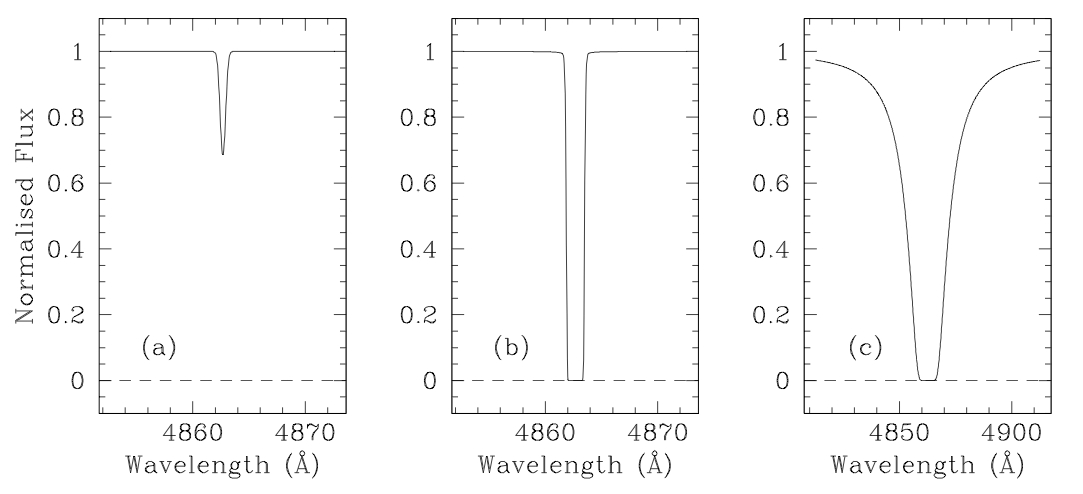
\includegraphics[scale=0.35, angle=0.0]{fig_linetypes.jpg}
\caption{\textsl{Examples of linear (a), saturated (b), and damped (c) absorption lines. All of these lines are Ly$\alpha$ lines redshifted to $z_{abs}=3.0$, with $b = 20$~km/s. $\log N(H~\text{{\sc i}}) = 13 ({\rm a}), 16 ({\rm b}), 20 ({\rm c})$}}\label{fig:linetypes}
\end{center}
\end{figure}
\end{center}

\begin{center}
\begin{figure}[htbp]
\begin{center}
% scale and angle values to be adjusted
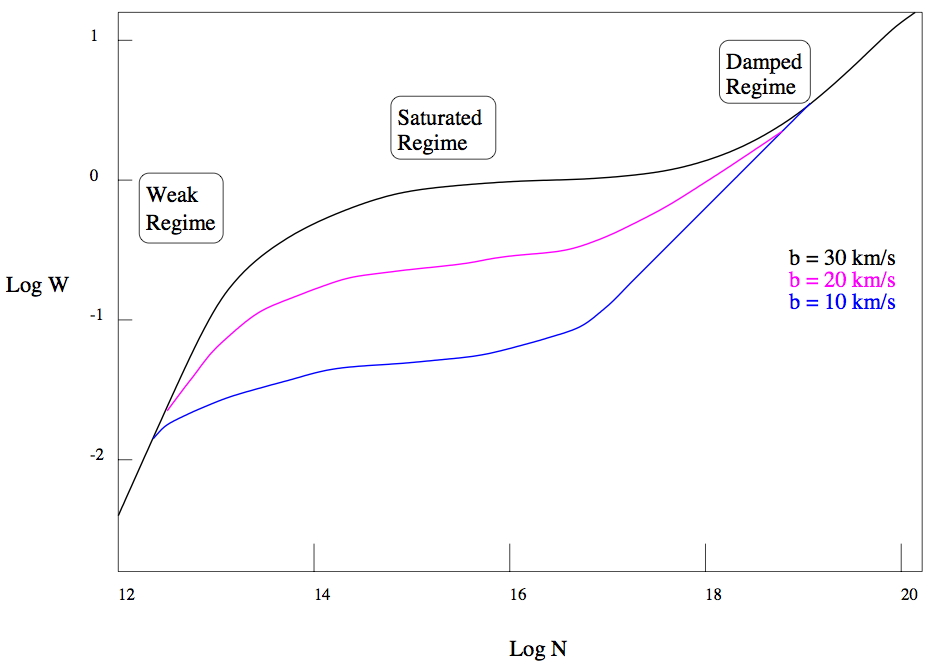
\includegraphics[scale=0.28, angle=0.0]{fig_cog.jpg}
\caption{\textsl{Schematic figure illustrating the curve of growth for Ly$\alpha$ absorption lines for three different $b$-values (Doppler widths).}}\label{fig:cog}
\end{center}
\end{figure}
\end{center}

\section{Redshift}

Another very important concept in spectroscopy, and astronomy in general, is finding how far away an object is. This can be done by calculating the object's redshift. In order to do this properly, one must know the wavelength at which an element emits/absorbs here at Earth (the rest wavelength) and the wavelength the object in space is emiting that same element (the observed wavelength). From there it is a simple calculation:
\begin{equation}
    z = \frac{\lambda_{obs} - \lambda_r}{\lambda_r} = 1 - \frac{\lambda_{obs}}{\lambda_r}
\end{equation} 

where $\lambda_{obs}$ is the observed wavelength from the object and $\lambda_r$ is the rest wavelength. At non-relativistic speeds this can be approximated to:
\begin{equation}
    z \approx \frac{v_r}{c}
\end{equation}

which gives you an idea of how fast an object is moving away from you.

For objects such as galaxies, sometimes it is possible to calculate the rotation curve as well by using these simple equations. Instead of using the rest wavelength here at Earth, define the center of the galaxy--the bulge is usually the brightest part--to be the rest frame and the opposite edges of the galaxies to be the observed wavelengths. This is just one of many fun examples of ways spectroscopy helps do amazing science.


Redshift increases both $W$ and FWHM by a factor of $(1 + z)$, which may sometimes result in an otherwise unresolved line being resolved (and which will also mean that, even for constant SNR, the detection limit on a line will depend on that line's redshift).

\section{Relative Solar Abundances}

Elemental abundances are often expressed in solar-relative terms, denoted by surrounding the element with square brackets, as shown below:
\begin{equation}
	[Z] = log(N(Z)/N(H)) - log(N(Z)/N(H))_\odot
\end{equation}
Thus, [Zn] = -1.0 would mean that the Zinc is 1/10 as abundant \emph{when compared to hydrogen} in the system of interest as compared to the solar system. In many astronomical systems, it is assumed that N(H)$\sim$N(H~{\sc i}), and that the abundance of the dominant ionization state of the element involved (e.g. Zn~{\sc ii} for zinc) is essentially equal to the abundance of that element as a whole.

Note that solar system abundances may be measured either in the solar atmosphere or in meteoroids, and that these values do not always agree exactly. Note also that, when a pure logarithmic abundance relative to hydrogen is expressed, it may have 13 added to it (by convention, when quoting solar abundances log(X/H) = log(X/H) + 13.00). This won't matter when computing the solar-relative abundance, but is worth knowing so as to avoid confusion.

Relative abundances are also used to compare different metals. For example, [Cr/Zn] is used as a measure of dust abundance because Cr depletes onto dust grains whereas Zn generally does not.

